\newcommand{\sflow}{\begin{itemize}}
\newcommand{\eflow}{\end{itemize}}
\newcommand{\sub}[2]{\item \textbf{{S-#1} #2}}
\newcommand{\af}[2]{\item \textbf{{E-#1} #2}}

\section{Use Cases}
\begin{center}
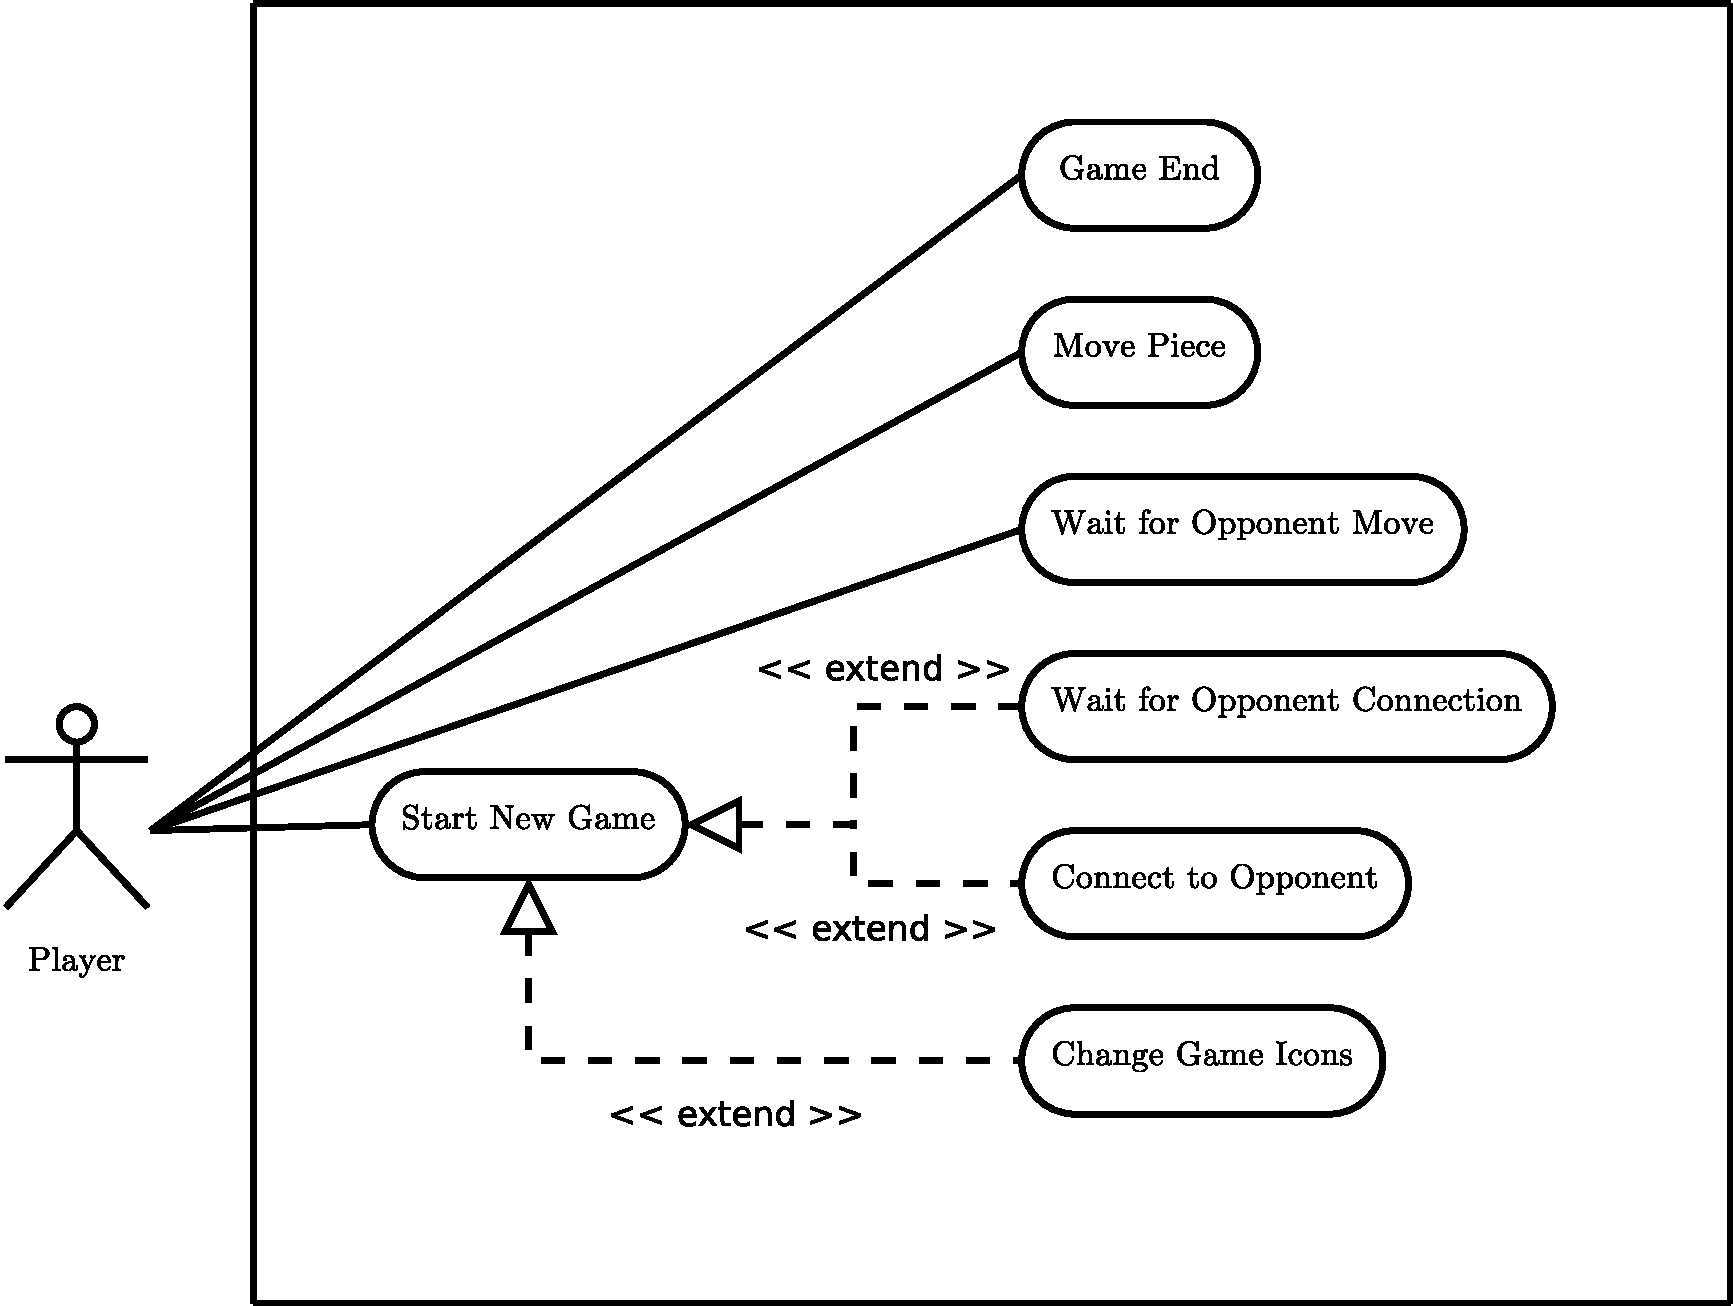
\includegraphics[scale=0.5]{usecase.pdf}
\end{center}

\subsection{Start New Game}
\subsubsection*{Preconditions}
None.
\subsubsection*{Main Flow}
The use case begins when the system presents the player with a connection dialog containing two methods of play (S-1).
The user may choose icons for the chess pieces (S-2). The system then attempts to establish a connection to the remote
player (S-3, E-1).
\subsubsection*{Subflows}
\sflow
\sub{1}{Method Selection}
The player shall select either ``Wait for an Opponent'' or ``Connect to an Opponent.'' Waiting for an opponent moves the
system to the ``Wait for Opponent Connection'' use-case. ``Connect to Opponent'' moves the system to the ``Connect to
Opponent'' use-case.
\sub{2}{Icon Selection}
The player shall have the ability to select ``Change Game Icons'' before starting the game. Doing so will move the system
to the ``Change Game Icons'' use-case.
\sub{3}{Connection}
The player shall select ``Ok'' in the connection dialog to either wait for an incoming player connection or attempt to
establish a connection based on the selection of S-1.
\eflow

\subsubsection*{Alternative Flows}
\sflow
\af{1}{Connection Failure}
The program was unable to establish a connection. The system presents a dialog explaining the cause of the error shall
be shown and return to the connection dialog.
\af{2}{Program Closed}
The program has been closed and the program shall terminate.
\eflow

\subsection{Wait for Opponent Connection}
\subsubsection*{Preconditions}
The user has selected ``Wait for an Opponent'' in the ``Begin Game'' use-case and pressed ``Ok.''
\subsubsection*{Main Flow}
The system shall prevents further actions (S-1) until another user connects (S-2).
\subsubsection*{Subflows}
\sflow
\sub{1}{Connection Dialog Lock}
The user shall not be able to interact with the connection dialog until a connection is established.

\sub{2}{User Connects}
Another user connects to the system (as specified in the ``Connect to Opponent'' use-case.) The game board shall be
shown and the connection dialog hidden and the system moves to the ``Move Piece'' use-case.
\eflow

\subsubsection*{Alternative Flows}
\sflow
\af{1}{Program Closed}
The program has been closed and the program shall terminate.
\eflow

\subsection{Connect to Opponent}
\subsubsection*{Preconditions}
The user has selected ``Connect to an Opponent'' in the ``Begin Game'' use-case and pressed ``Ok.''
\subsubsection*{Main Flow}
The system shall attempt to connect to the specified IP and port (S-1). The connection may succeed (S-2)
or fail (E-1).
\subsubsection*{Subflows}
\sflow
\sub{1}{Attempt Connection}
The system shall attempt to establish a connection to the designated IP
and port. If successful, the system moves to (S-2). If unsuccessful, the system moves to
(E-1).
\sub{2}{Connection Successful}
The system shall display the board, hide the connection dialog and move
to the ``Wait for Opponent Move'' use-case.
\eflow
\subsubsection*{Alternative Flows}
\sflow
\af{1}{Connection Error}
There was an error with the connection or the connection timed out while
waiting for a response from the user. The game presents an error message and returns to the ``Start
New Game'' use-case.
\eflow

\subsection{Move Piece}
\subsubsection*{Preconditions}
It is the local user's turn.
\subsubsection*{Main Flow}
The user selects a piece and the system highlights the allowed moves on the board (S-1). The player then drags-and-drops
a piece onto an allowed square (S-2). This information is communicated to the remote player (S-3). If the move is not
allowed, the system goes to (E-1). In the case of network problems on either end, (E-2) is triggered.

\subsubsection*{Subflows}
\sflow
\sub{1}{Highlight Moves}
The user shall click a piece. The positions on the chess board that are allowed
for the selected piece shall be highlighted by changing to a different color.
\sub{2}{Allowed Move}
The user shall drag the piece onto an allowed position. The icon for the associated
piece shall be moved to that location by the system.
\sub{3}{Communicate Move}
The move shall be communicated to the remote system to update the remote chess board.
\eflow
\subsubsection*{Alternative Flows}
\sflow
\af{1}{Invalid Move}
The player has moved the piece to a disallowed position. The piece shall be moved
back to the original location by the system.

\af{2}{Network Error}
If either players' network connection fails, the game shall terminate.
\eflow

\subsection{Wait for Opponent Move}
\subsubsection*{Preconditions}
It is the remote player's turn.
\subsubsection*{Main Flow}
The remote player is making a move (use-case ``Move Piece'' from their perspective). The local board is
locked (S-1) and the player cannot move. Upon receiving a move from the opponent (S-2), the local system
moves to the ``Move Piece'' use-case.
\subsubsection*{Subflows}
\sflow
\sub{1}{Game Board Lock}
The game board shall be locked and the user is prevented from interacting
with the board or game pieces.
\sub{2}{Receive Move}
The remote user has moved (use-case ``Move Piece'' use-case from their perspective) and the local system shall move to
the ``Move Piece'' use-case if a win is not found. If it is, the system shall move to ``Game End.''
\eflow
\subsubsection*{Alternative Flows}
\sflow
\af{1}{Network Error}
If either players' network connection fails, the game shall terminate.
\eflow

\subsection{Game End}
\subsubsection*{Preconditions}
The game has been won by either player (S-1),
\subsubsection*{Main Flow}
Both players' boards shall be locked (S-1) and notified of who won (S-2). The game will then terminate.
\subsubsection*{Subflows}
\sflow
\sub{1}{Game Board Lock}
The game board shall be locked and the user prevented from interacting
with the board or game pieces.
\sub{2}{Win Notification}
Both players shall be notified of which player won the game. An ``Ok'' button shall be displayed which terminates the
game when clicked.
\eflow
\subsubsection*{Alternative Flows}
None.

\subsection{Change Game Icons}
\subsubsection*{Preconditions}
The user has selected ``Browse'' in the ``Custom Icon Directory'' box on the connection dialog.
\subsubsection*{Main Flow}
The user selects a directory on the local machine (S-1) and the dialog closes (S-2).
\subsubsection*{Subflows}
\sflow
\sub{1}{Directory Selection}
The user shall select a directory from their local machine containing icons
for the chess pieces.
\sub{2}{Dialog Close}
The system shall close the dialog and load the icons. The user shall be returned to
the connection dialog.
\eflow
\subsubsection*{Alternative Flows}
None.
